\section{CPU-level Energy Measurements}
\label{sec:energymeasure}

\begin{figure}[tbh]
    \centering
    \input{figs/test_setup.tex}
    \caption{Bench setup for measuring single instruction current drain}
    \label{fig:setup}
\end{figure}

High precision instruction level energy models can be derived for pipelined
processors by monitoring the instantaneous current drawn by the processor at
each clock cycle, as explained in \cite{nikolaidis2005instruction}. Modern
processors commonly operate at a few GHz, and Nyquist sampling theorem
\cite{nyquist1928certain} states that the sampling frequency must be twice the
frequency of the signal being measured. The signal sampled from the processor
might change at least once every clock cycle, so a cycle accurate measurement
would require very expensive instruments.

In \cite{rundehvatum2013exploring}, single instructions was measured by
exploting fast-loop-mode and looping over a group of equal instructions. An
Agilent bench multimeter and a shunt resistor was set up like shown in
\autoref{fig:setup}. This method provides an average power consumption when the
pipeline is (mostly) filled with a single type of instruction. Instead of normal
serial connected ammeter, the power rail is connected in series with a shunt
resistor equal to the one figured in \autoref{fig:shunt}, and voltage drop over
this resistor is measured using a voltmeter. This method provides a way to
measure currents either outside the range of the ammeter or with greater
accuracy. An example of how a shunt resistor can provide greater accuracy; when
an Agilent 34410A is used to measure a current in which the voltage exeeds 0.8V,
the readings is within 0.1\% when the system is correctly calibrated. If a shunt
resistor with the right characteristics is used, the voltage drop across the
shunt resistor will lie in the range 0 -- 100 mV, and then readings will,
according to the datasheet, be within 0.003\% \cite{agilent34410a}.

\begin{figure}[tbh]
    \centering
    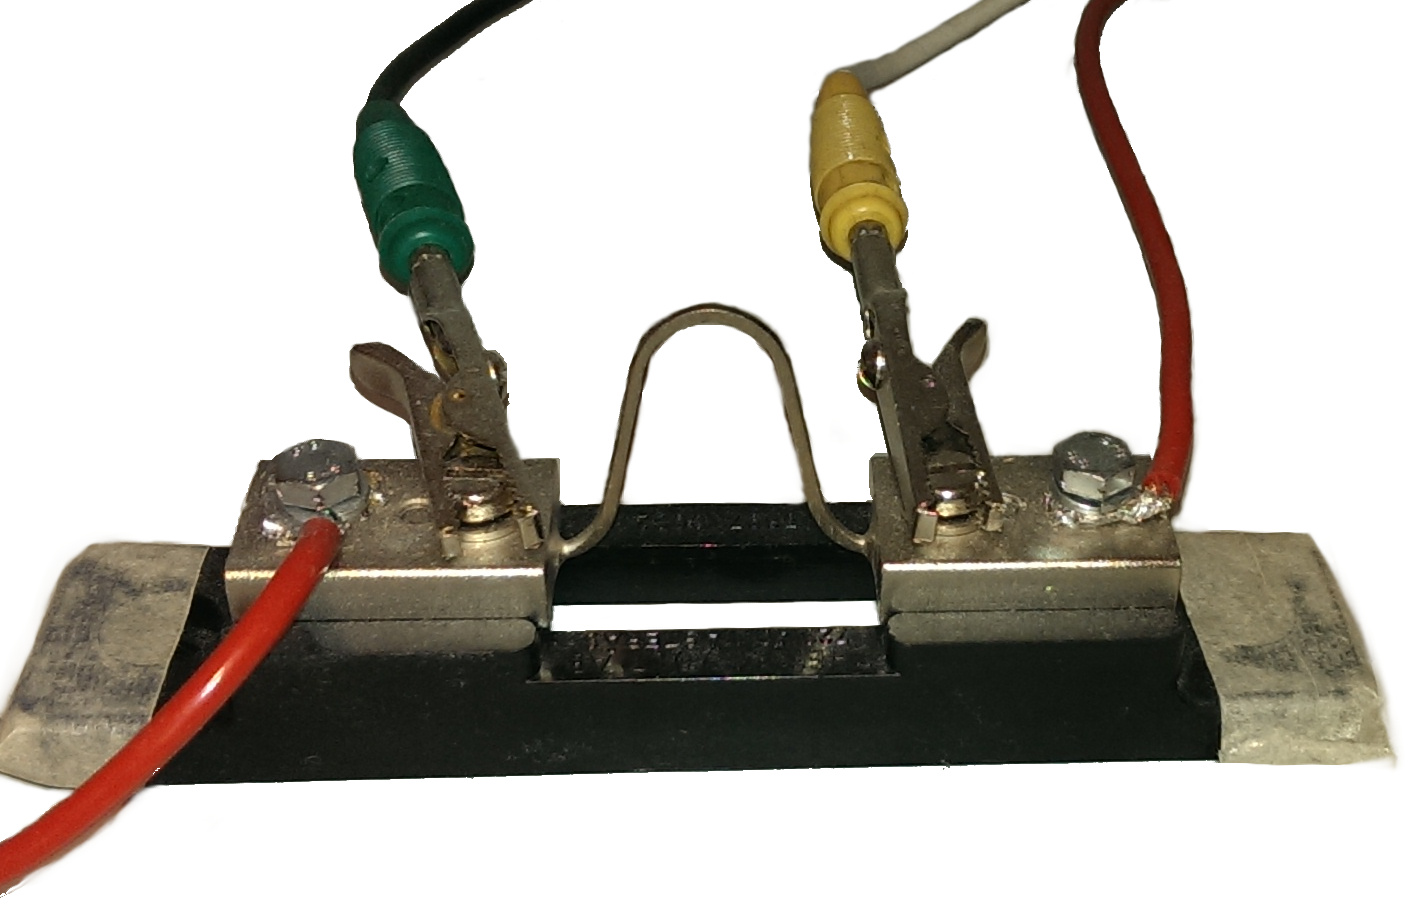
\includegraphics[width=0.8\textwidth]{figs/shunt.jpg}
    \caption{An example shunt resistor}
    \label{fig:shunt}
\end{figure}

% TODO: Where does this fit?
% The ultimate goal in this context is to estimate power consumption and energy
% efficiency of new hardware, the first step is to measure different more or less
% power consuming events on real hardware that is similar to the one simulated.

